\chapter{Desenvolvimento de aplicativos móveis} \label{cap:referencialteorico} 

DIZER COMO EH EM RELACAO AO DESENVOLVIMENTO NORMAL DE SOFTWARE
-> 3.1. Challenges of mobile applications development: http://www.sciencedirect.com/science/article/pii/S2090447915001276

%TOPICO 3 http://ac.els-cdn.com/S2090447915001276/1-s2.0-S2090447915001276-main.pdf?_tid=80a952a8-2a87-11e6-b99c-00000aacb360&acdnat=1465067395_ac6fb22ebd08d76bc6f9add4b2543d64

%aqui serão descritos as diferencas sucintamente enre nativo e cross
%explicar as diferencas
% Referencias boas para leitura
% http://www.teclogica.com.br/blog/desenvolvimento-para-dispositivos-moveis-nativo-x-cross-platform/ 
% http://pt.slideshare.net/suelengc/nativo-vs-crossplataform
% https://www.ibm.com/developerworks/community/blogs/ctaurion/entry/desenvolvimento_de_apps-parte_2_hibrido_nativo_ou_web?lang=en
% http://blog.concretesolutions.com.br/2016/03/nativo-x-hibrido/
% http://martinfowler.com/articles/multiMobile/#cost

\section{Desenvolvimento Nativo} \label{section:desenvolvimentonativo}

Aplicações nativas são desenvolvidas com o uso de ferramentas e linguagens de programação específicas para determinada plataforma, usando o \textit{SDK} e \textit{frameworks} providos por ela. Os \textit{apps} ficam vinculados a esse ambiente, executando apenas nos dispositivos da plataforma alvo \cite{kassas_taxonomy_2015}. Caso haja a necessidade de implementação para múltiplas plataformas, a aplicação deve ser desenvolvida separadamente para cada uma delas \cite{heitkotter_evaluating_2013}.
%para cada um dos ambientes
%para cada uma das plataformas
%Dado que

Posto que o \textit{app} é desenvolvido em ambiente próprio, segue-se os padrões técnicos, de interface e de experiência de usuário determinados pela plataforma, provendo um \textit{look and feel} de aplicação nativa ao usuário.
Aplicações nativas tem fácil acesso, por meio de APIs fornecidas pelas plataformas, a recursos dos dispositivos móveis, como sensores, câmera, GPS, contatos e e-mail \cite{kassas_taxonomy_2015}.

Nas seções a seguir serão descritas as arquiteturas das plataformas \textit{iOS} e \textit{Android}, duas das plataformas mais conhecidas e utilizadas para desenvolvimento nativo de aplicações \textit{mobile} \cite{jobe_native_2013}.

\subsection{iOS} \label{subsection:ios}

O sistema operacional \textit{iOS} foi lançado juntamente com o primeiro \textit{iPhone} criado em Janeiro de 2007 e 
funciona como uma interface entre as aplicações desenvolvidas pelos programadores (\textit{apps}) e o \textit{hardware} 
dos dispositivos (\textit{iPhone}, \textit{iPad}, \textit{iPod}) \cite{apple_inc_apple_2007}. 
Dessa forma, a comunicação com o \textit{hardware} do dispositivo se dá 
por meio de um conjunto bem definido de interfaces do sistema, o que facilita o desenvolvimento de \textit{apps} 
que funcionam entre os variados tipos de \textit{hardware} dos dispositivos da Apple \cite{apple_inc_developing_2016}. 

Como recomendação, a Apple explica que deve-se preferir o uso de camadas mais elevadas, pois as camadas de 
mais alto nível possuem abstrações orientadas à objeto de funcionalidades das camadas mais baixas. Isso 
torna o desenvolvimento mais fácil, pois reduz a quantidade de código que deve ser criado e mantém funcionalidades 
complexas das camadas mais baixas encapsuladas por meio das interfaces. No entanto, não há problema em usar 
funcionalidades presentes nas camadas mais baixas, se essas não estiverem disponíveis por meio de abstrações nas 
camadas superiores \cite{apple_inc_tech_2014}. 

A maioria das interfaces disponíveis para uso são disponibilizadas por meio de \textit{frameworks}, 
que são diretórios, que podem ser adicionados ao projeto no \textit{Xcode}, contendo \textit{DSL's} e os recursos necessários como, 
imagens, aplicativos auxiliares e arquivos \textit{header}, para o \textit{framework} funcionar corretamente \cite{apple_inc_tech_2014}.

\subsubsection{Arquitetura \textit{iOS}} \label{subsubsection:arc-ios}
Sua arquitetura é baseada nas camadas listadas, conforme a Figura~\ref{fig:arc-ios}, a seguir.
 
\begin{figure}[H]
  \centering
    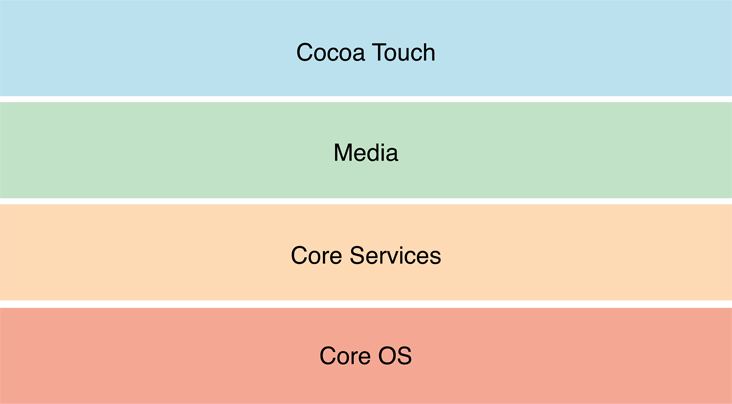
\includegraphics[width=0.5\textwidth]{arc-ios}
    \caption[Arquitetura iOS]{ Arquitetura iOS. Fonte: \cite{apple_inc_tech_2014}.}
	\label{fig:arc-ios}
\end{figure}

As camadas do \textit{iOS} são explicadas com mais detalhes a seguir.
 
\begin{itemize}
	\item A camada \textit{Cocoa Touch} é a camada mais alto nível onde são fornecidos serviços básicos de interação 
    com o usuário como entrada baseada em toques e notificações \textit{Push} e outras tecnologias necessárias para
     melhorar a experiencia do usuário como multitarefas, Continuidade (\textit{Handoff}) e \textit{AirDrop}, além de \textit{frameworks} 
     de alto nível que permitem acesso a funcionalidades do sistema como \textit{AddressBook} para contatos, \textit{EventKit} 
     para eventos relacionados ao calendário e \textit{MapKit} para mapas \cite{apple_inc_tech_2014}.
	\item A camada logo abaixo da \textit{Cocoa Touch} é a camada \textit{Media} que contém tecnologias e \textit{frameworks} necessários 
    para a implementação de experiências multimídia com áudio, vídeo e gráficos \cite{apple_inc_tech_2014}.
	\item A próxima camada, logo abaixo da camada \textit{Media}, é a camada \textit{Core Services}. Essa camada está mais próxima 
    do \textit{hardware} e portanto possui acesso a funcionalidades de mais baixo nível como localização, telefonia, \textit{threads} 
    e \textit{SQLite}. Aqui residem dois dos \textit{frameworks} mais importantes do \textit{iOS} que são o \textit{Foundation} e o \textit{Core Foundation}, 
    ambos relacionados com o gerenciamento de dados e alguns serviços e definem todos os tipos básicos de dados que 
    todos os \textit{apps} usam, como por exemplo, coleções, \textit{strings}, data e hora, \textit{sockets} e \textit{threads} \cite{apple_inc_tech_2014}.
	\item A última camada é a camada \textit{Core OS}, na qual as funcionalidades de mais baixo nível são construídas e 
    provavelmente utilizadas por outros \textit{frameworks} em outras camadas. Se a aplicação possui requisitos de segurança 
    ou comunicação com acessórios externos mais complicados, é possível usar as funcionalidades dessa camada \cite{apple_inc_tech_2014}.
\end{itemize}

\subsubsection{Desenvolvimento \textit{iOS}} \label{subsubsection-dev-ios}

O kit de desenvolvimento da plataforma (SDK) \textit{iOS} permite que os desenvolvedores criem suas aplicações e a testem em emuladores. 
Contudo, para que os testes sejam realizados em um dispositivo é exigida uma licença do \textit{Apple Developer Program}, 
com custo de US\$99,00 anuais. A licença também é necessária para a utilização de recursos avançados e para a distribuição 
na \textit{App Store}, loja de aplicativos da Apple \cite{apple_inc_program_2016}.   

Para a distrituição de aplicativos \textit{iOS}, além da licença citada, é necessário submeter a aplicação para avaliação e aprovação da Apple antes de ir para a App Store. Para agilizar o processo de aprovação, é necessário que o aplicativo esteja de acordo com as diretrizes estabelecidades pela Apple, como as orientações de interface gráfica e as orientações de revisão da App Store \cite{apple_inc_submitting_2016}.

Desenvolver aplicativos para a plataforma iOS requer um computador com o sistema operacional Mac OS e o ambiente de desenvolvimento Xcode \cite{heitkotter_evaluating_2013}. 
O desenvolvimento é atrelado a duas linguagens de programação, o \textit{Objective-C} e o \textit{Swift}.
O Objective-C constitui-se em um superconjunto da linguagem de programação C, da qual herda a maior parte da sua sintaxe, incluindo tipos primitivos e fluxo de declarações, e adiciona sintaxe própria para definição de classes e métodos \cite{apple_inc_about_2014}. 
%É uma linguagem que teve origem nos anos 80 e ganhou destaque junto ao crescimento da Apple.
O \textit{Swift} foi lançado pela Apple como um sucessor do \textit{Objective-C}. É uma linguagem gratuita, código aberto e pode ser integrada a códigos \textit{Objective-C} \cite{apple_inc_swift_2016}. Pouco tempo após o seu lançamento, tornou-se uma das linguagens de programação mais utilizadas no mundo \cite{rebouas_empirical_2016}. Segundo a Apple, o \textit{Swift} possui uma sintaxe concisa, além de ser intuitivo e poderoso \cite{apple_inc_swift_2016}.

\subsection{Android} \label{subsection:android}

O sistema operacional \textit{Android} foi criado pela \textit{start-up} homônima Android Inc. em outubro de 2003. Em agosto de 2005 foi adquirida pela empresa Google, que lançou
em novembro de 2007, juntamente com a OHA, o sistema \textit{Android}, \textit{open-source} e baseado no \textit{kernel} do Linux. Uma semana depois, foi liberada a primeira versão do \textit{SDK} para \textit{Android}.
O sistema foi concebido originalmente para camêras fotográficas, no entanto, foi percebido por seus criadores um mercado maior no ramo da telefonia e desviou-se o 
foco para \textit{smartphones}, competindo diretamente com Symbian e Windows Mobile.

\subsubsection{Arquitetura \textit{Android}} \label{subsection:arc-android}

A arquitetura Android é baseada nas camadas apresentadas na Figura~\ref{fig:arc-android} e são explicadas com mais detalhes a seguir.

\begin{itemize}
%http://source.android.com/devices/index.html <- Fonte principal
%traduzir e parafrasear

    \item A camada mais elevada é a \textit{Application Framework}, onde as aplicações construídas pelos desenvolvedores são instaladas \cite{android_android_2016}.
    \item A camada logo a abaixo da \textit{Application Framework} é a \textit{Binder IPC Proxies}, onde \textit{IPC} significa \textit{Inter-Process Comunication}.
    É a camada que faz uma ponte entre as aplicações instaladas na camada superior com a próxima camada, a \textit{System Services}. É uma interface que permite que \textit{API's}
    de alto nível interajam com serviços do sistema que residem na camada abaixo dela \cite{android_android_2016}. 
    \item Abaixo da \textit{Binder IPC Proxies} fica a \textit{System Services}, que , por meio de módulos, permite acesso a \textit{hardwares} específicos. Cada serviço presente nessa camada,
    foi desenvolvido para gerenciar um componente específico, como busca e notificações. Os serviços foram divididos em duas categorias, \textit{Media} e \textit{System}, explicadas a seguir \cite{android_android_2016}.
    \begin{itemize}
        \item \textit{Media Server}: são os serviços responsáveis por gerenciar conteúdos de mídia como gravação e reprodução de audio e vídeo. 
        \item \textit{System Server}: são serviços responsáveis por gerenciar os demais tipos de serviço do sistema como notificações e \textit{windows}.
    \end{itemize}
    \item Abaixo da camada \textit{System Services} fica a camada \textit{HAL} que permite que fornecedores de \textit{hardware} criem interfaces e \textit{drivers} para os \textit{hardwares} que
    ele oferecem. Com isso, é possível criar novas funcionalidades e implementá-las sem afetar o resto das camadas do sistema \cite{android_android_2016}.  
    \item A camada mais baixa é a \textit{Linux Kernel} que é uma versão do \textit{kernel} do Linux com algumas modificações como uma gerenciamento de memória mais avançados e próprio para dispositivos 
    móveis e funcionalidades para dispositivos embarcados \cite{android_android_2016}. 
    
\end{itemize}

\begin{figure}[h]
  \centering
    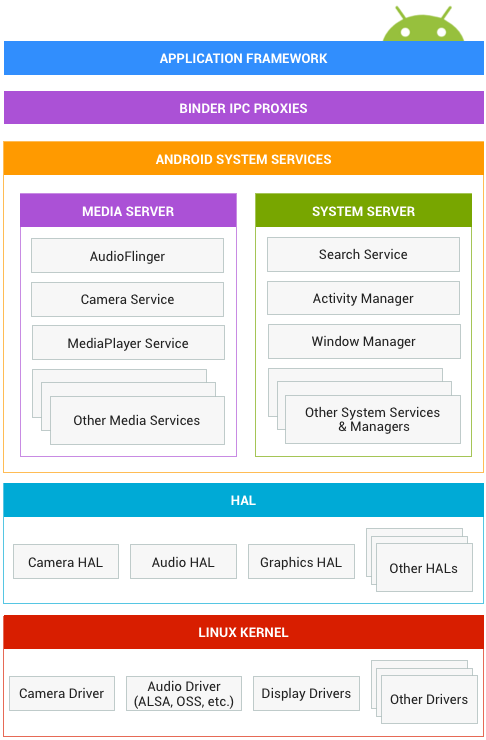
\includegraphics[width=0.5\textwidth]{arc-android}
    \caption[Arquitetura Android]{ Arquitetura Android. Fonte: \cite{android_android_2016}.}
	\label{fig:arc-android}
\end{figure}

\subsubsection{Desenvolvimento \textit{Android}} \label{subsection:dev-android}

Para o desenvolvimento de aplicações \textit{Android} é necessário conhecimento na linguagem de programação Java.
Não é requerido sistema operacional específico e a IDE recomendada pelo Google é o \textit{Android Studio}, oficial para desenvolvimento de aplicativos \textit{Android} \cite{android_meet_2016}.
%O ambiente necessário para o desenvolvimento requer um computador com qualquer sistema operacional e o \textit{Android Studio}, a \textit{IDE} oficial para a criação de aplicativos Android \cite{android_meet_2016}.

Para a publicação na loja de aplicativos do Google, \textit{Google Play Store}, é cobrada uma taxa única de US\$25. 
Antes de serem publicados, os aplicativos passam por um processo de revisão para assegurar que não violam as políticas estabelecidas pela loja \cite{meier_creating_2015}.  

\section{Desenvolvimento \textit{Cross-platform}} \label{section:desenvolvimentomulti}

solucoes cross-platform auxiliam no desenvolvimento

escrever um codigo e rodam a aplicacao em diferentes plataformas
\cite{kassas_taxonomy_2015}

desenvolvimento com um ambiente e deployment em mvarias plataformas

Para desenvolver uma aplicacao nativa que rode em diferentes plataformas, seria necessario criar uma para cada plataforma, o que exige tempo, investimento, equipe com conhecimento nas variadas tecnologias usadas pelas plataformas alvo.

Solucao surgiu os webapps e as aplicações híbridas.

\textcolor{red}{relacionar com linha de produto}

\textit{Web apps} são aplicações implementadas utilizando tecnologias \textit{web}, levando em conta aspectos intrínsecos aos dispositivos móveis, como tamanho de tela e modo de uso \cite{heitkotter_evaluating_2013}. Segundo \citeonline{stark_building_2010}, \textit{web apps} não são instalados no dispositivo e não ficam disponíveis nas lojas de aplicativos, em vez disso, são acessados pelos \textit{browsers} dos dispositivos. \textit{Web apps} não possibilitam o uso de alguns recursos de hardware dos dispositivos como sensores e GPS \cite{heitkotter_evaluating_2013}. Conforme \citeonline{heitkotter_evaluating_2013}, \textit{web apps} costumam ter a aparência e o comportamento de páginas \textit{web} comuns, divergindo dos elementos de tela padrão providos pelas plataformas \textit{mobile}.

A abordagem híbrida surgiu como uma combinação do uso das tecnologias web junto à possibilidade de acesso à funcionalidades nativas \cite{heitkotter_evaluating_2013}.
Em essência, aplicações híbridas são \textit{web sites} inseridos em um wrapper...



%http://www.ymedialabs.com/hybrid-vs-native-mobile-apps-the-answer-is-clear/

crossapps sao apps desenvolvidos uitlizando recnologias web que suportam multiplas plataformas moveis, podem ser webapps ou hybrids.



\subsection{PhoneGap e Cordova} \label{subsection:phonegap}

\textit{PhoneGap} é um \textit{framework} para desenvolvimento de aplicativos híbridos, criado pela empresa Nitobi. 
Após a empresa ser comprada pela Adobe Systems Inc. o \textit{PhoneGap} teve seu código doado para a Apache Software Foundation 
para garantir que outras empresas pudessem contribuir, já que muitas empresas já conheciam as licenças da Apache \cite{bezerra_desenvolvimento_2016}.


Como o \textit{PhoneGap} é uma marca registrada de propriedade da Adobe, na Apache teve seu nome alterado para Cordova.
Tanto o \textit{Apache Cordova} quanto o \textit{Adobe PhoneGap}, são gratuitos e \textit{open sources}, no entanto, o 
\textit{PhoneGap} possui um ambiente integrado com serviços da Adobe como o \textit{PhoneGap Build}, por exemplo \cite{bezerra_desenvolvimento_2016}.
 
\textit{Cordova} permite que aplicações não nativas tenham acesso a funcionalidades nativas do dispositivo como sensores, 
contatos e câmera. No entanto, o Cordova apenas consegue fazer um aplicativo criado em 
\textit{HTML} rodar como se fosse nativo em um dispositivo com \textit{Android} e \textit{iOS}, mas não consegue 
imitar a usabilidade e aparência dos dispositivos nativos \cite{bezerra_desenvolvimento_2016}. 

Para preencher essa lacuna, outros \textit{frameworks} foram criados em cima do Cordova como um complemento, 
provendo bibliotecas \textit{HTML} e \textit{CSS} para a 
criação de um \textit{front-end} que se aproxime o máximo possível da usabilidade e experiência de usuário de 
aplicações móveis nativas \cite{bezerra_desenvolvimento_2016}.

O \textit{Cordova} possui muitos plugins para poder acessar funcionalidades específicas do aparelho em que está sendo 
executado. Esses devem ser instalados no projeto do aplicativo via \textit{CLI} \cite{bezerra_desenvolvimento_2016}. 

A fim de se evitar confusões em relação aos nomes dados ao \textit{PhoneGap} e ao \textit{Cordova}, pode-se entender o \textit{PhoneGap} 
como uma distribuição do \textit{Apache Cordova}, mantido pela Adobe Systems Inc. 

%(http://ddd.uab.cat/pub/tfg/2014/tfg_5062/article.pdf phonegap)

%https://www.quora.com/What-is-the-difference-between-PhoneGap-and-Cordova-and-why-would-I-select-one-over-another
%http://luisvasconcellos.com/2015/04/06/apps-hibridas-com-cordova-e-ionic.html
%https://www.quora.com/What-is-the-difference-between-Cordova-and-Ionic
%https://en.wikipedia.org/wiki/Apache_Cordova
%http://cordova.apache.org/docs/en/latest/guide/overview/

\subsection{AngularJS} \label{subsection:angularjs}

\textit{HTML} é a principal linguagem de marcação para a criação de páginas \textit{web}. No entanto, os conteúdos 
exibidos são estáticos e o \textit{HTML} não fornece suporte para conteúdos dinâmicos.
\textit{AngularJS} é um \textit{framework open source}, mantido pelo Google, que permite extender a sintaxe do 
\textit{HTML} para poder criar páginas \textit{web} com conteúdos dinâmicos \cite{bezerra_desenvolvimento_2016}.

Com ele é possível utilizar \textit{tags} não nativas do \textit{HTML} para gerenciar conteúdos que ainda não 
foram dispostos na tela, ou seja, o usuário faz uma ação por meio da interface gráfica, 
o AngularJS interpreta a ação e faz uma requisição para o servidor pedindo apenas o conteúdo necessário, que é 
diferente do que já está sendo mostrado para o usuário. 
O servidor retorna o conteúdo específico e o AngularJS apresenta o novo conteúdo inserindo-o corretamente junto 
com o antigo já mostrado (https://angularjs.org/).
\textcolor{red}{FAZER IMAGEM EXPLICATIVA DO FUNCIONAMENTO DO ANGULAR}

Foi projetado para criação de \textit{SPA's} e com isso faz com que as páginas sejam mais rápidas, visto que, apenas é carregado o conteúdo que precisa ser mostrado, 
deixando outros conteúdos para serem carregados dinâmicamente depois, de acordo com as interações do usuário.

%(Diseño e implementación de una aplicación multidispositivo en un entorno HTML5, Alvaro Martínez Rodríguez, fala que é feito para SPAs).
%(http://ddd.uab.cat/pub/tfg/2015/tfg_7125/Articulo-TFG_2.0.pdf)


%(http://www.barbiana20.unirc.it/wp-content/uploads/2015/07/Tesi-Cristiano-finale-2.pdf , artigo italiano fala muito bem explicado a origem do angularjs)
%(\textcolor{red}{ESTE ARTIGO ESTA OTIMO PARA CRIAR A IMAGEM QUE EU QUERO BASEADA NA IMAGEM DELE DA PAGINA 33, OU COLOCAR A IMAGEM DELE E CITAR ELE DIRETAMENTE})
%(tbm fala que é feito para SPAs, pagina 54)



\subsection{Ionic} \label{subsection:ionic}

NESTA SEÇÃO e do \textit{Ionic Framework}, usado para desenvolvimento multiplataformas e \textit{frameworks} necessários para o correto funcionamento do \textit{Ionic}...

%http://blog.ionic.io/how-2015-went-for-ionic/
\textit{Ionic} é um \textit{framework} gratuito e \textit{open source} para desenvolvimento de aplicativos híbridos utilizando tecnologias 
\textit{web} como \textit{HTML}, \textit{CSS} e \textit{JavaScript} otimizadas para dispositivos móveis. 


Foi criado pela empresa Drifty Co. em 2013 com base na necessidade que seus clientes apresentavam de criarem \textit{apps}. 
Foi projetado para ser muito performático e funcionar com padrões e tecnologias \textit{web} modernas. 


Criado sobre os \textit{frameworks} \textit{Cordova} e \textit{AngularJS}, com apenas um código é possível criar aplicativos para várias 
plataformas como \textit{iOS} e \textit{Android}, por exemplo, dentre outras. O \textit{Ionic} conta ainda com um conjunto de ferramentas para auxiliar 
no desenvolvimento dos aplicativos.

\subsubsection{Arquitetura de um projeto Ionic} \label{subsubsection:arc-ionic}

%http://mcgivery.com/structure-of-an-ionic-app/
Um projeto \textit{Ionic} pode ser dividido em cinco camadas, listadas e detalhadas a seguir.

\begin{itemize}
    \item \textit{Views}: São a camada de apresentação, onde as informações são mostradas para o usuário. Pode ser comparada como 
    o seu homônimo no padrão \textit{MVC}. Muitas vezes são chamadas de \textit{templates}, pois é a forma com o AngularJS 
    se refere a elas. São, normalmente, arquivos \textit{HTML} separados, que são chamados e inseridos quando necessário pelo
    AngularJS. É possível utilizar \textit{data binding} nas Views para poder estabelecer uma conexão com a controladora
    e compartilhar informações entre as duas camadas.
    \item \textit{Controllers}: É a camada responsável por controlar o fluxo de dados e lógica da aplicação. Também pode ser
    comparada com a camada homônima no padrão \textit{MVC}. Ela é responsável por apresentar ao usuário as Views e chamar as camadas
    de dados (\textit{Services/Factories}) para ligar os dados reais da aplicação, por meio de \textit{data binding}, à interface
    gráfica. As controladoras possuem uma variável chamada \textit{scope}, que possui todas as informações que são necessárias 
    para a criação da View.
    \item \textit{Data(Services/Factories)}: É a camada que se aproxima da camada \textit{model} do padrão \textit{MVC}. Encapsula
    dados da aplicação e provê esses dados, geralmente, por meio de um \textit{web service}. Essa camada responde às requisições
    da controladora com os dados a serem utilizados para a criação da View e para serem mostrados para o usuário. 
    \item \textit{App Configuration}: Nesta camada, as controladoras são ligadas às suas interfaces por meio de rotas. É possível
    também, criar rotas padrão, para o caso de não haver nenhuma rota que esteja sendo identificada o sistema não quebrar.
    \item \textit{Directives}: Essa camada serve para especificar comportamentos específicos em elementos de uma página 
    \textit{HTML}, ou seja, elas são um elemento ou um atributo que podem iniciar um comportamento específico definido 
    pelo programador. É possível, por exemplo, criar uma diretiva para sempre colocar uma imagem padrão caso uma validação 
    retorne um valor falso.  
\end{itemize}

\subsubsection{Desenvolvimento \textit{Ionic}} \label{subsubsection:dev-ionic}
Para o desenvolvimento de aplicações utilizando \textit{Ionic}, não é necessário nenhum equipamento específico, assim como no desenvolvimento \textit{Android}.
...

É necessário apenas um computador com qualquer sistema operacional

No entanto, para o desenvolvimento do app \textit{iOS}, ainda é necessário que se possua um computador com Mac OS e com o Xcode.
...

Pode-se utilizar qualquer \textit{IDE} de acordo com as preferências do programador.
...

A linguagem utilizada é o \textit{JavaScript}, usando ainda \textit{HTML} e \textit{CSS}....


\subsubsection{Ferramentas de Apoio} \label{subsection:ionicferramentasapoio}

O \textit{Ionic} provê além do \textit{HTML} e \textit{CSS} otimizado para dispositivos móveis, 
uma série de ferramentas, que compõem um ecossistema de apoio, que fornecem velocidade e facilidade no desenvolvimento de aplicativos híbridos. 
Essas ferramentas são listadas a seguir com uma breve explicação do que cada uma pode fazer \cite{drifty_ionic:_2013}.

\begin{itemize}

    \item \textbf{Ionic Framework}: É o \textit{framework front-end} para criação de aplicativos híbridos com tecnologias \textit{web} construído em cima
    do \textit{Apache Cordova}. Facilita a criação de aplicativos com interface gráfica e interações muito semelhantes aos dispositivos nativos, de modo que 
    a experiência de usuário não seja diferente no uso de uma aplicação nativa e multiplataforma \cite{drifty_ionic:_2013}. 
    
    \item \textbf{Ionic Creator}: Com essa ferramenta \textit{on-line} é possível criar protótipos funcionais utilizando \textit{drag and drop}
    , que podem ser executados em dispositivos ou simuladores, e depois exportar o projeto criado para a 
    inserção de lógicas de negócio. Ela é gratuita para teste, ou seja, é possível criar um protótipo e fazer o \textit{download}
    do código para continuar o desenvolvimento, no entanto, no momento em que este trabalho foi conduzido, só era possível
    fazer a pré-visualização em dispositivos reais para usuários pagantes \cite{drifty_ionic_2016}.
    
    \item \textbf{Ionic Lab}: É uma ferramenta \textit{desktop} para testar o projeto que está sendo criado com o \textit{Ionic}. Nela é possível
    executar o projeto em templates prontos de \textit{iOS} e \textit{Android}, rodar os simuladores de cada plataforma,
    gerenciar plugins do \textit{Cordova} e ver um console com \textit{logs} relativos à execução do projeto. Encapsula o \textit{CLI} do \textit{Ionic} com uma interface gráfica simples
    e intuitiva \cite{drifty_ionic_2015}.
    
    \item \textbf{Ionic Playground}: É uma ferramenta \textit{on-line} para criar e testar códigos \textit{HTML}, \textit{CSS} e \textit{JavaScript} 
    já integrado com a plataforma \textit{AngularJS}. Nela é possível editar códigos nas três linguagens citadas e ver em tempo real as alterações 
    feitas aparecerem dentro de um \textit{template} de dispositivo móvel, sem a necessidade de salvar, compilar ou executar o projeto e sem ter que 
    configurar o ambiente necessário para o desenvolvimento \cite{drifty_ionic_2016-2}. 
    
    \item \textbf{Ionic View App}: É um aplicativo disponível para as plataformas \textit{iOS} e \textit{Android} onde é possível testar o 
    aplicativo criado no \textit{Ionic} diretamente em um dispositivo real como se fosse nativo. É possível compartilhar os projetos criados para serem
    testados por clientes e testadores sem a necessidade de passar pelas lojas de aplicativos de cada plataforma. É semelhante ao serviço 
    \textit{Testflight} da Apple para testar aplicativos, ainda em desenvolvimento, e receber \textit{feedbacks} dos clientes e testadores que o testarem \cite{drifty_ionic_2016-3}.
    
    \item \textbf{Ionic Platform}: É a plataforma \textit{on-line} do \textit{Ionic} que possui serviços de \textit{back-end} em nuvem para análise de dados de uso,
     usuários, configuração de \textit{Push Notifications}, criação dos pacotes nativos e dar \textit{deploy} nas aplicações criadas sem a necessidade de
     resubmeter o aplicativo para as respectivas lojas \cite{drifty_ionic_2016-1}. 
     
\end{itemize}

\section{Comparativo (Nativo x \textit{Cross-platform})} \label{section:comparativo}

% LEMBRAR DE POR COMO VANTAGEM DO CROSS: FASTER(INITIAL) SPEED TO MARKET
% Esse site faz um comparativo muito bom... http://www.ymedialabs.com/hybrid-vs-native-mobile-apps-the-answer-is-clear/
%gostei da conclusao a que ele chegou da escolha de nativo ou hibrido!

% e cita dados interessantes e informacoes como
% o facebook era hibrido e depois veio pro nativo
% o instagram demorou 2 anos pra desenvolver a versao android (questao: sera que realmente % é necessario lançar mais de uma plataforma ao mesmo tempo?)

Cada plataforma possui seu próprio ambiente de desenvolvimento, arquitetura, ferramentas, mercado de distribuição e público alvo \cite{shakshuki_4th_2013}.
E cada abordagem de desenvolvimento possui suas características próprias e inerentes à forma como se dá o projeto, desenvolvimento e distribuição dos \textit{apps} \cite{corral_ant_2012}.

Algo importante que deve ser feito pela equipe de desenvolvimento é decidir para qual plataforma desenvolver, tendo sempre em vista que 
ao não criar o aplicativo para uma plataforma, uma grande parcela do mercado pode estar sendo desconsiderada, o que acaba por reduzir o alcance
da aplicação e por consequência os lucros obtidos com o \textit{app} \cite{corral_ant_2012}. 

Para o desenvolvimento de várias aplicações para cada plataforma de maneira nativa, é preciso passar por todo o processo de desenvolvimento novamente, 
pois para cada plataforma há uma arquitetura distinta que deve ser seguida, padrões de código e interface de usuário e \textit{API's} próprias \cite{holzinger_making_2012}.
Dessa forma, cada aplicação deve ser codificada considerando as diferentes arquiteturas, componentes e \textit{guidelines}, customizadas o máximo possível 
para ser a mesma aplicação em plataformas distintas e por fim, gerados novos executáveis e distribuídos nas diferentes lojas de aplicativos \cite{corral_ant_2012}.

Isso implica em planejar cada \textit{app} com base em uma plataforma distinta, por mais que se trate do mesmo aplicativo, o que acaba por encarecer 
e tornar mais lento o desenvolvimento \cite{kassas_taxonomy_2015}. Por exemplo, existem componentes que não existem em todas as arquiteturas (\textit{navigationController} e 
\textit{tabBarController} presentes na plataforma \textit{iOS}, por exemplo) e que devem ser considerados no projeto do \textit{app} para as demais plataformas \cite{shakshuki_4th_2013}.

No entanto, quando se pensa em desenvolvimento multiplataformas, o projeto se torna agnóstico em relação à plataforma, pois o projeto é feito pensando-se 
apenas em uma arquitetura, um ambiente de desenvolvimento e um conjunto único de ferramentas e não de acordo com as características de cada plataforma. Após o desenvolvimento do núcleo da
aplicação, podem ser feitas customizações para adaptar melhor o aplicativo para cada plataforma alvo da distribuição, criando assim um produto final verdadeiramente multiplataformas \cite{corral_ant_2012}.
%Dessa forma, a equipe de desenvolvedores pode focar nos requisitos da aplicação sem se preocupar tanto com as diferenças entre plataformas.
%essa frase depende da referencia ser encontrada

A Figura~\ref{fig:dev-natxcross} mostra as diferenças no processo de desenvolvimento de um \textit{app} utilizando tecnologias \textit{cross-plataform} e 
nativas.

\begin{figure}[H]
  \centering
    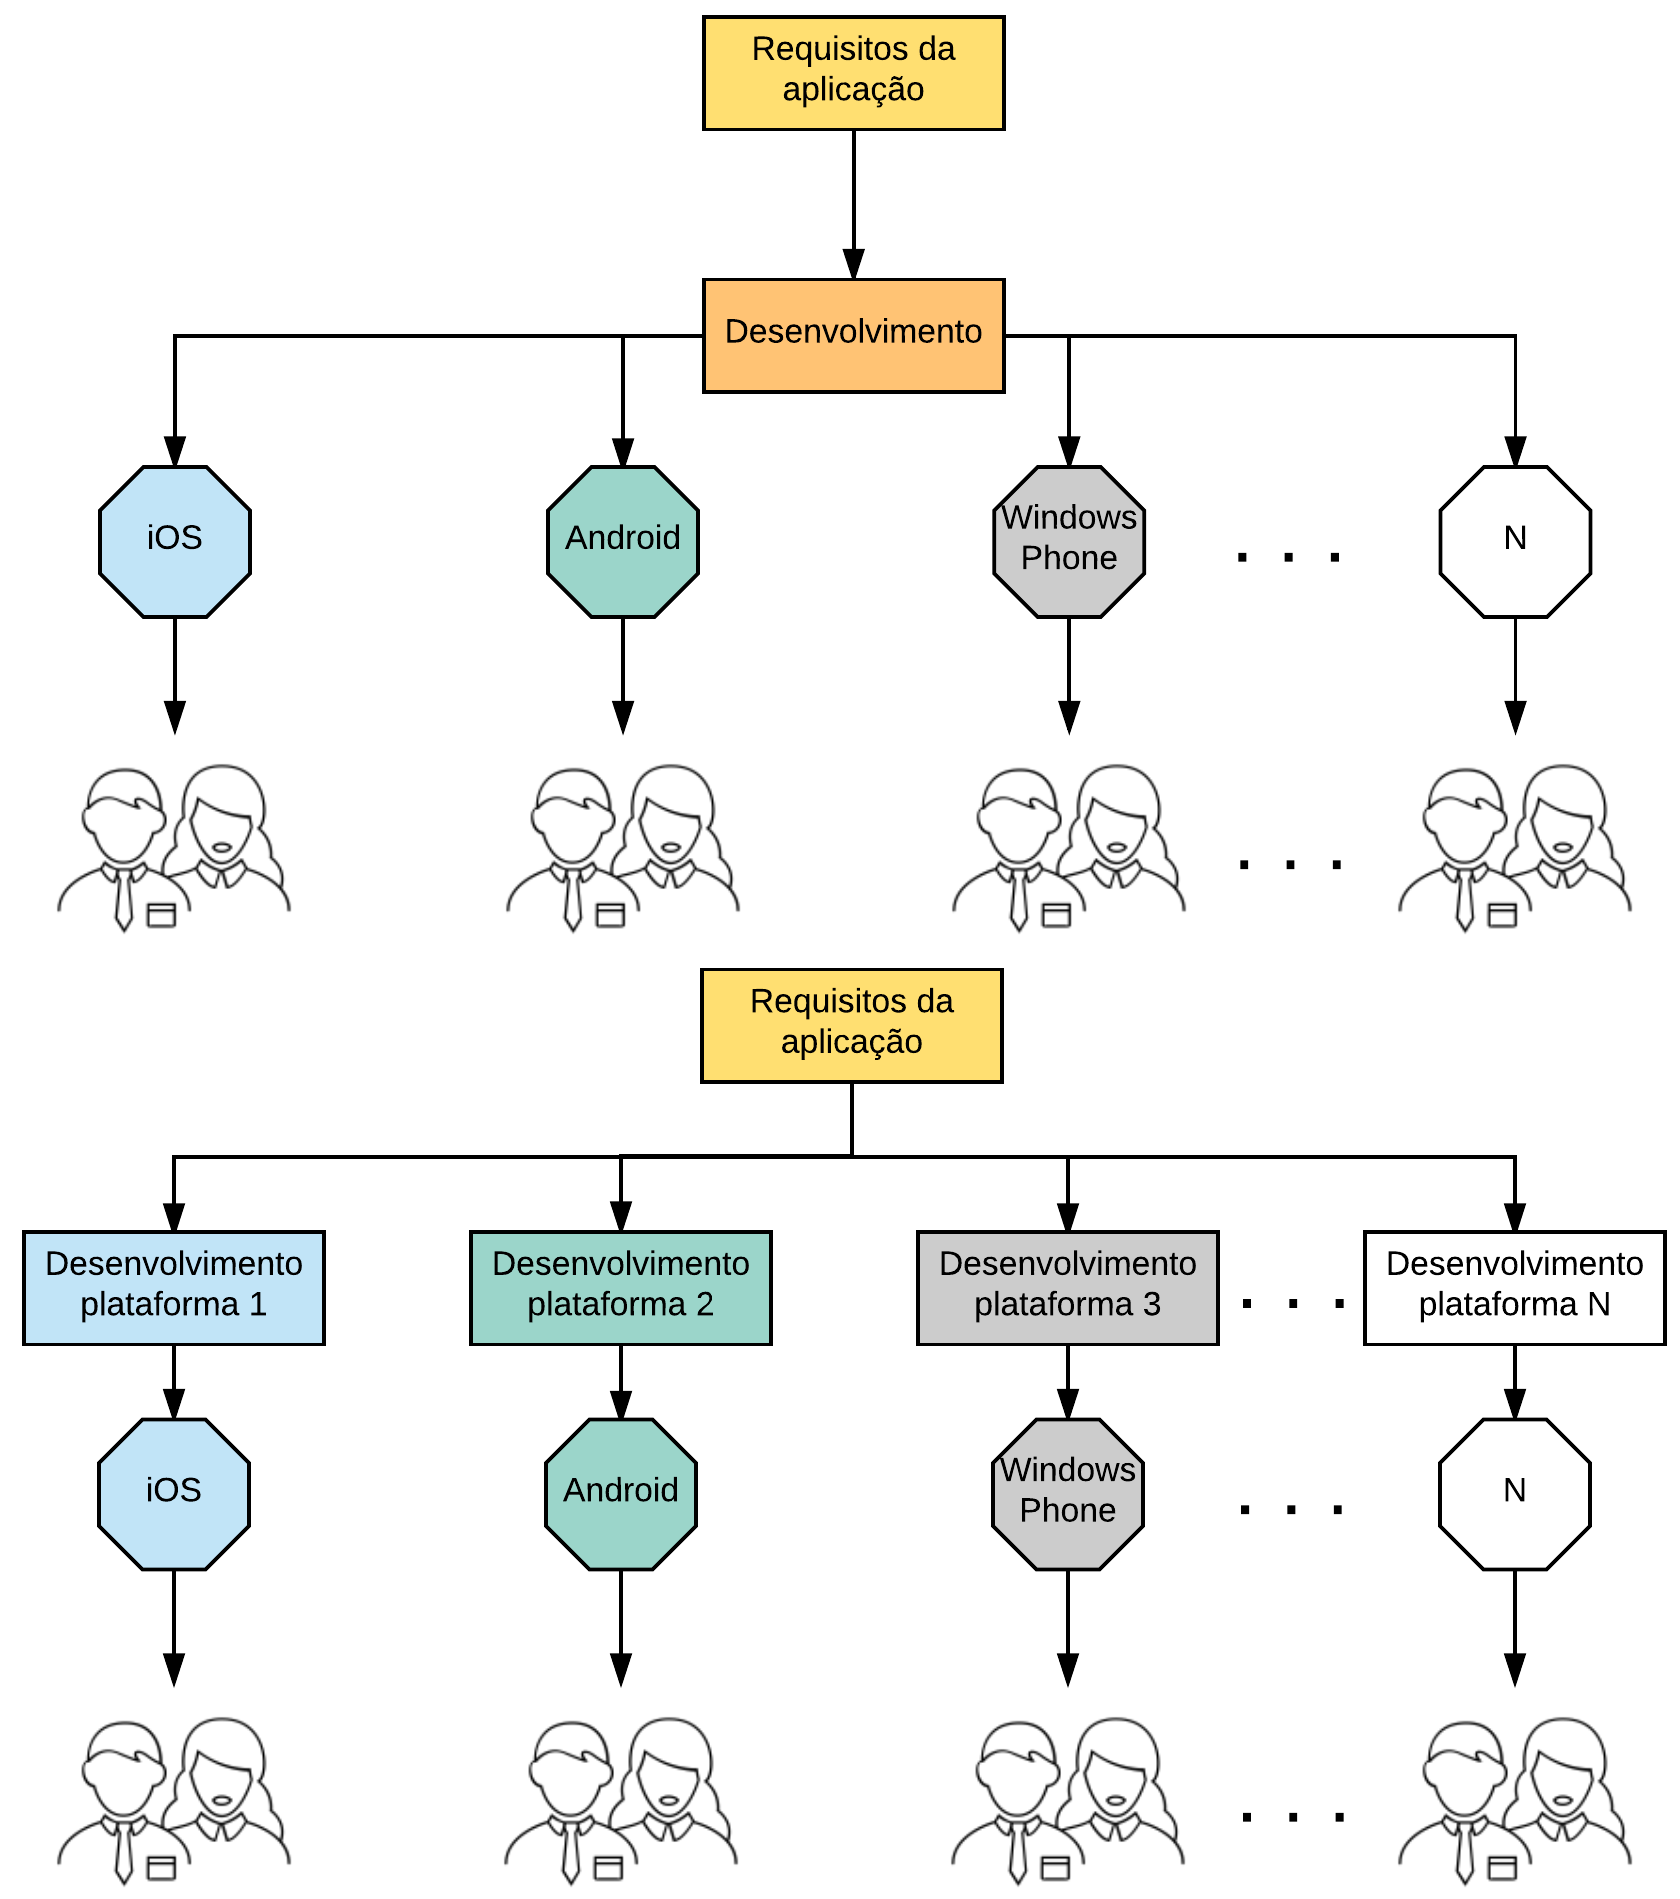
\includegraphics[width=1.0\textwidth]{dev-natxcross}
    \caption[Desenvolvimento \textit{Cross-plataform} x Nativo]{ Desenvolvimento \textit{Cross-plataform} x Nativo. Fonte: Baseado em \cite{corral_ant_2012}}
	\label{fig:dev-natxcross}
\end{figure}

A Tabela~\ref{vantxdesva} sumariza as principais vantagens e desvantagens de cada tipo de desenvolvimento para uma melhor compreensão de cada abordagem.

\textcolor{red}{AQUI TEM UMA TABELA!!}